%\section{Motivation}
In this chapter copper foils are first chemically polished and prepared for investigation in SEM (p. \pageref{fig:SEM-gb}), AFM (p. \pageref{fig:foil-afm-as-bought}) and STM (p. \pageref{fig:cu-foil-clean-stm}). After CVD growth of \textit{h}-BN with borazine, foils are investigated in XPS (compare \autoref{fig:xps-self-grown}) and STM (\autoref{fig:h-bn-overgrown-cu}). A comparison to bought \textit{h}-BN foils is found at the end of the chapter.

%Comparable experiments  are performed by \cite[8]{stables_report_2008}). 

	\section{Pre-treatment of Cu-foils: Polishing}
	
	\paragraph{Experiment realization}The first attempt to etch the Cu-foil was performed with the $5\%_{vol}$ EG, $25\%_{vol}\,H_2O$ filled up with phosphoric acid. The etching was performed in a \SI{200}{\ml} beaker, filled with \SI{150}{\ml} etching solution. The potential was adjusted to be \SI{1.2}{\V} during the polishing process. The current through the solution changes and is typically highest when the polishing process started (\SI{120}{\milli \ampere}). 
	
	After some minutes the foils reflectivity changes. The foils surface - shiny before etching - becomes hazy. After some more time the foils reflectivity improves again. 
	
	The time spend for polishing depends on the handling (like shaking the beaker or moving the foil in the solution). When no visual change to the surface is observed the etching process is interrupted. 
	%\footnote{Since the perfect voltage/current to perform polishing varies in time a automated etching process has been developed \cite{palmieri_besides_2001}}
	
	One has to be careful if reproducible results are needed. During the etching process (as more and more copper settles on the counter electrode), the current and therefore the etching rate decreases continuously. When the beaker is moved, some of the debris on the electrode changes (the electrode's) surrounding and the etching rate (limiting current) increases again. 
	Front- and backside of the foil are suspect to different etching processes. The back side is generally more flat, the side facing the counter electrode always shows some additional protrusions.
	
	\paragraph{After etching treatment}
	The foil is taken out and cleaned from remaining etchants with purified water first and isopropanol afterwards. Foils are be stored in isopropanol to avoid oxidation.
	
%	\paragraph{SEM}
%	\label{sec:foil-SEM}
%	\input{./includes/chapter/sem-technique}
	
	\begin{figure}\centering
		\subfigure[\SI{570}{\micro \meter}$\times$\SI{380}{\micro \meter}]{\includegraphics[width=0.45\textwidth]{./images/Domenik_16031715}
			\label{fig:SEM-1}
			
		} \quad
		\subfigure[\SI{18}{\micro \meter}$\times$\SI{12}{\micro \meter}]{\includegraphics[width=0.45\textwidth]{./images/Domenik_16031717}
			\label{fig:SEM-2}
		} \quad
		\subfigure[\SI{5.6}{\micro \meter}$\times$\SI{3.7}{\micro \meter}]{\includegraphics[width=0.45\textwidth]{./images/Domenik_16031700}
			\label{fig:SEM-3}
		}
		\caption{SEM image of etched copper foil. Different contrast suggests different grain-orientation within the surface. \subref{fig:SEM-1} Larger image showing the contrast of different grains in the copper-foil, \subref{fig:SEM-2} zoom to an area with two different contrasts and their border. \subref{fig:SEM-3} A dark grain is embedded in an otherwise curly surface. On both, bright small features are visible and attributed to an inhomogeneous etching process. Recorded with U=\SI{5}{\kilo \eV}}
		\label{fig:SEM-gb}
	\end{figure}
	
	\paragraph{SEM characterization} One can see in \autoref{fig:SEM-gb} that the surface is imaged in different intensities. These are attributed to the different orientation of the copper grains within the foil\cite{wu_effects_2015}. The grain size ranges from just a few \SI{}{\micro \meter} to several hundred \SI{}{\micro \meter}. 
	
	Large grains are preferred for growing graphene on copper foils because grain boundaries are subject to inhomogeneities within the graphene layer and provide a route for unwanted surface chemistry (copper oxidation for example). This effect can also be used to highlight grain boundaries as shown in \cite{wu_effects_2015}.
	
	The copper foil shows surface variation. While some areas of the sample show some wavy surface, whereas other are much flatter and appear in a different intensity (\autoref{fig:SEM-gb}).
	
	No estimation on the grains' facet orientation have been done due to the lack of EBSD-data in the SEM setup.
	
%	\begin{figure}[] \centering
%		\includegraphics[width=0.7\textwidth]{./images/Domenik_16031700.jpg}
%		%\includegraphics[height=6cm]{../Daten/SEM/160317-Domenik/Domenik_16031717.jpg}
%		\caption{Close up SEM image that shows different surface morphologies after polishing (\SI{5.6}{\micro \meter}$\times$\SI{3.7}{\micro \meter}). A dark grain is embedded in an otherwise curly surface. On both, bright small features are visible and attributed to an inhomogeneous etching process. Recorded with U=\SI{5}{\kilo \eV}}
%		\label{fig:SEM-surface}
%	\end{figure}
	
	\paragraph{RT-AFM}
	\label{sec:foil-AFM}
	To investigate the sample roughness AFM measurements are done at an AFM operated under ambient conditions.
	
	\begin{figure}\centering
		\subfigure[Copper foil before etching.]{
			\includegraphics[width=0.35\textwidth]{./images/as_bought0000}
			\label{fig:foil-bought-afm}
		} \quad
		\subfigure[Copper foil after etching]{
			\includegraphics[width=0.35\textwidth]{./images/polished0000}
			\label{fig:foil-polished-afm}
		} \quad
		\subfigure[Height profiles of the two samples.]{
			\includegraphics[width=0.7\textwidth]{./images/as_bought-polished_0000-profiles}
			\label{fig:foil-profiles}
		}
		\caption{RT-AFM topography image of copper foil as bought from Alfa Aesar \subref{fig:foil-bought-afm} before and \subref{fig:foil-polished-afm} after etching. \subref{fig:foil-profiles} Height profile averaging the lower 10 lines of \subref{fig:foil-bought-afm} and \subref{fig:foil-polished-afm}. Roughness along the line profiles decreases after etching ($Rq_{before}=\SI{7.3}{\nano \meter} \rightarrow Rq_{after}=\SI{3.6}{\nano \meter}$). Color scale for both AFM images \SI{100}{\nano \meter}, Image width: \SI{20}{\micro \meter}}.
		\label{fig:foil-afm-as-bought}
	\end{figure}
	
	Figure \ref{fig:foil-bought-afm} shows the striations that stem from the production process (from top to buttom).
	%\begin{figure}[] \centering
	%	\subfigure[RMS $\approx$\SI{9}{\nm} in the left image, contrast \SI{100}{\nm}]{
	%	\includegraphics[width=0.4\textwidth]{./images/polished0000.jpg}
	%}
	%	\subfigure[RMS $\approx$\SI{3}{\nm} in the right image, contrast \SI{70}{\nm}]{
	%	\includegraphics[width=0.4\textwidth]{./images/polished0001.jpg}
	%}
	%	\caption{AFM image of a copper foil polished 5h (according to table \ref{tab:used-etching-solution}), \textcolor{red}{\textbf{IMAGING PARAMETERS!}}}
	%	\label{fig:foil-afm-polished}
	%\end{figure}
	
	After etching ($U=1.2V$,I=\SIrange{120}{250}{\mA}) for \SI{5}{\hour} (spolution shown in table \ref{tab:used-etching-solution}) the striations have gone and the RMS value decreased by \SI{50}{\percent} and an increase in foil quality is obvious even with bare eyes. Figure \ref{fig:foil-afm-as-bought} show RT-AFM images in the same size and contrast - before \subref{fig:foil-bought-afm} and after \subref{fig:foil-polished-afm} etching.
	The circular hole is an effect of bubbles in the etching process where the bubble affects the rate of etching. The over all structure changes from a heterogenous sample height to a flat height contribution with only a little amount of defects. Those are sufficiently seperated in space to exhibit flat regions where the h-BN may grow unperturbated.
	
\subsection{LT-STM characterization}
\label{section:foil-STM}
The bought and chemically polished foils are mounted on a sample holder and loaded into the load lock. It is evacuated for \SIrange{2}{3}{\hour}, afterwards the valve is opened to the chamber. During transfer, no noteable increase in the base pressure is noted. The sample is put on the parking slot.
		
The sample was initially degassed with slowly increasing temperatures to remove adsorbates like $CO, CO_2$ and $H_2O$.
		
After some time of degassing, the sample was prepared with repeated sputter and anneal cycles. The annealing temperatures were increased up to \SI{800}{\degreeCelsius}. 
The sample was cooled down and observed in LT-STM.
		
Further experiments were carried out to increase the cleanliness of the \textit{h}-BN on the polycrystalline copper foil. To reduce the amount of elements coming from the body of the foil, it is repeatedly sputtered and annealed to temperatures as high as \SI{800}{\celsius}. This may have also an improving influence on the grain size and amount of corrugation. Several attempts have been made which are described in summary below.
%%%%%%%%%%%%%%%%%%%%%%%%%%%%%%%%%%%%%%%%%%%%%%%%%%%%%%%%%%%%%%%%%%%%%%%%%%%%%%%%%%%%%%%%%%
After cleaning, the sample is investigated in STM. The foil shows a inhomogeneous topography, with parts of the sample showing very flat regions while others still remain heavily corrugated and not scan able in STM.  A look onto the quite heterogeneous surface reveals flat areas with a typical roughness of $\approx \SI{70}{\pico\meter}$ exist (\autoref{fig:cu-foil-clean-stm-1}). Areas with very large corrugations $\geq \SI{100}{nm}$ are hard to scan in STM and bad places for \textit{h}-BN growth. Although being flat, the polycrystalline foil shows a lot of unordered substrate steps and a dirty surface, covered with adsorbates and crystal defects imaged as small bright dots.
%%%%%%%%%%%%%%%%%%%%%%%%%%%%%%%%%%%%%%%%%%%%%%%%%%%%%%%

\begin{figure}[] \centering
	%	\subfigure[Roughness $\approx \SI{60}{\pico\meter}$.]{%
	%		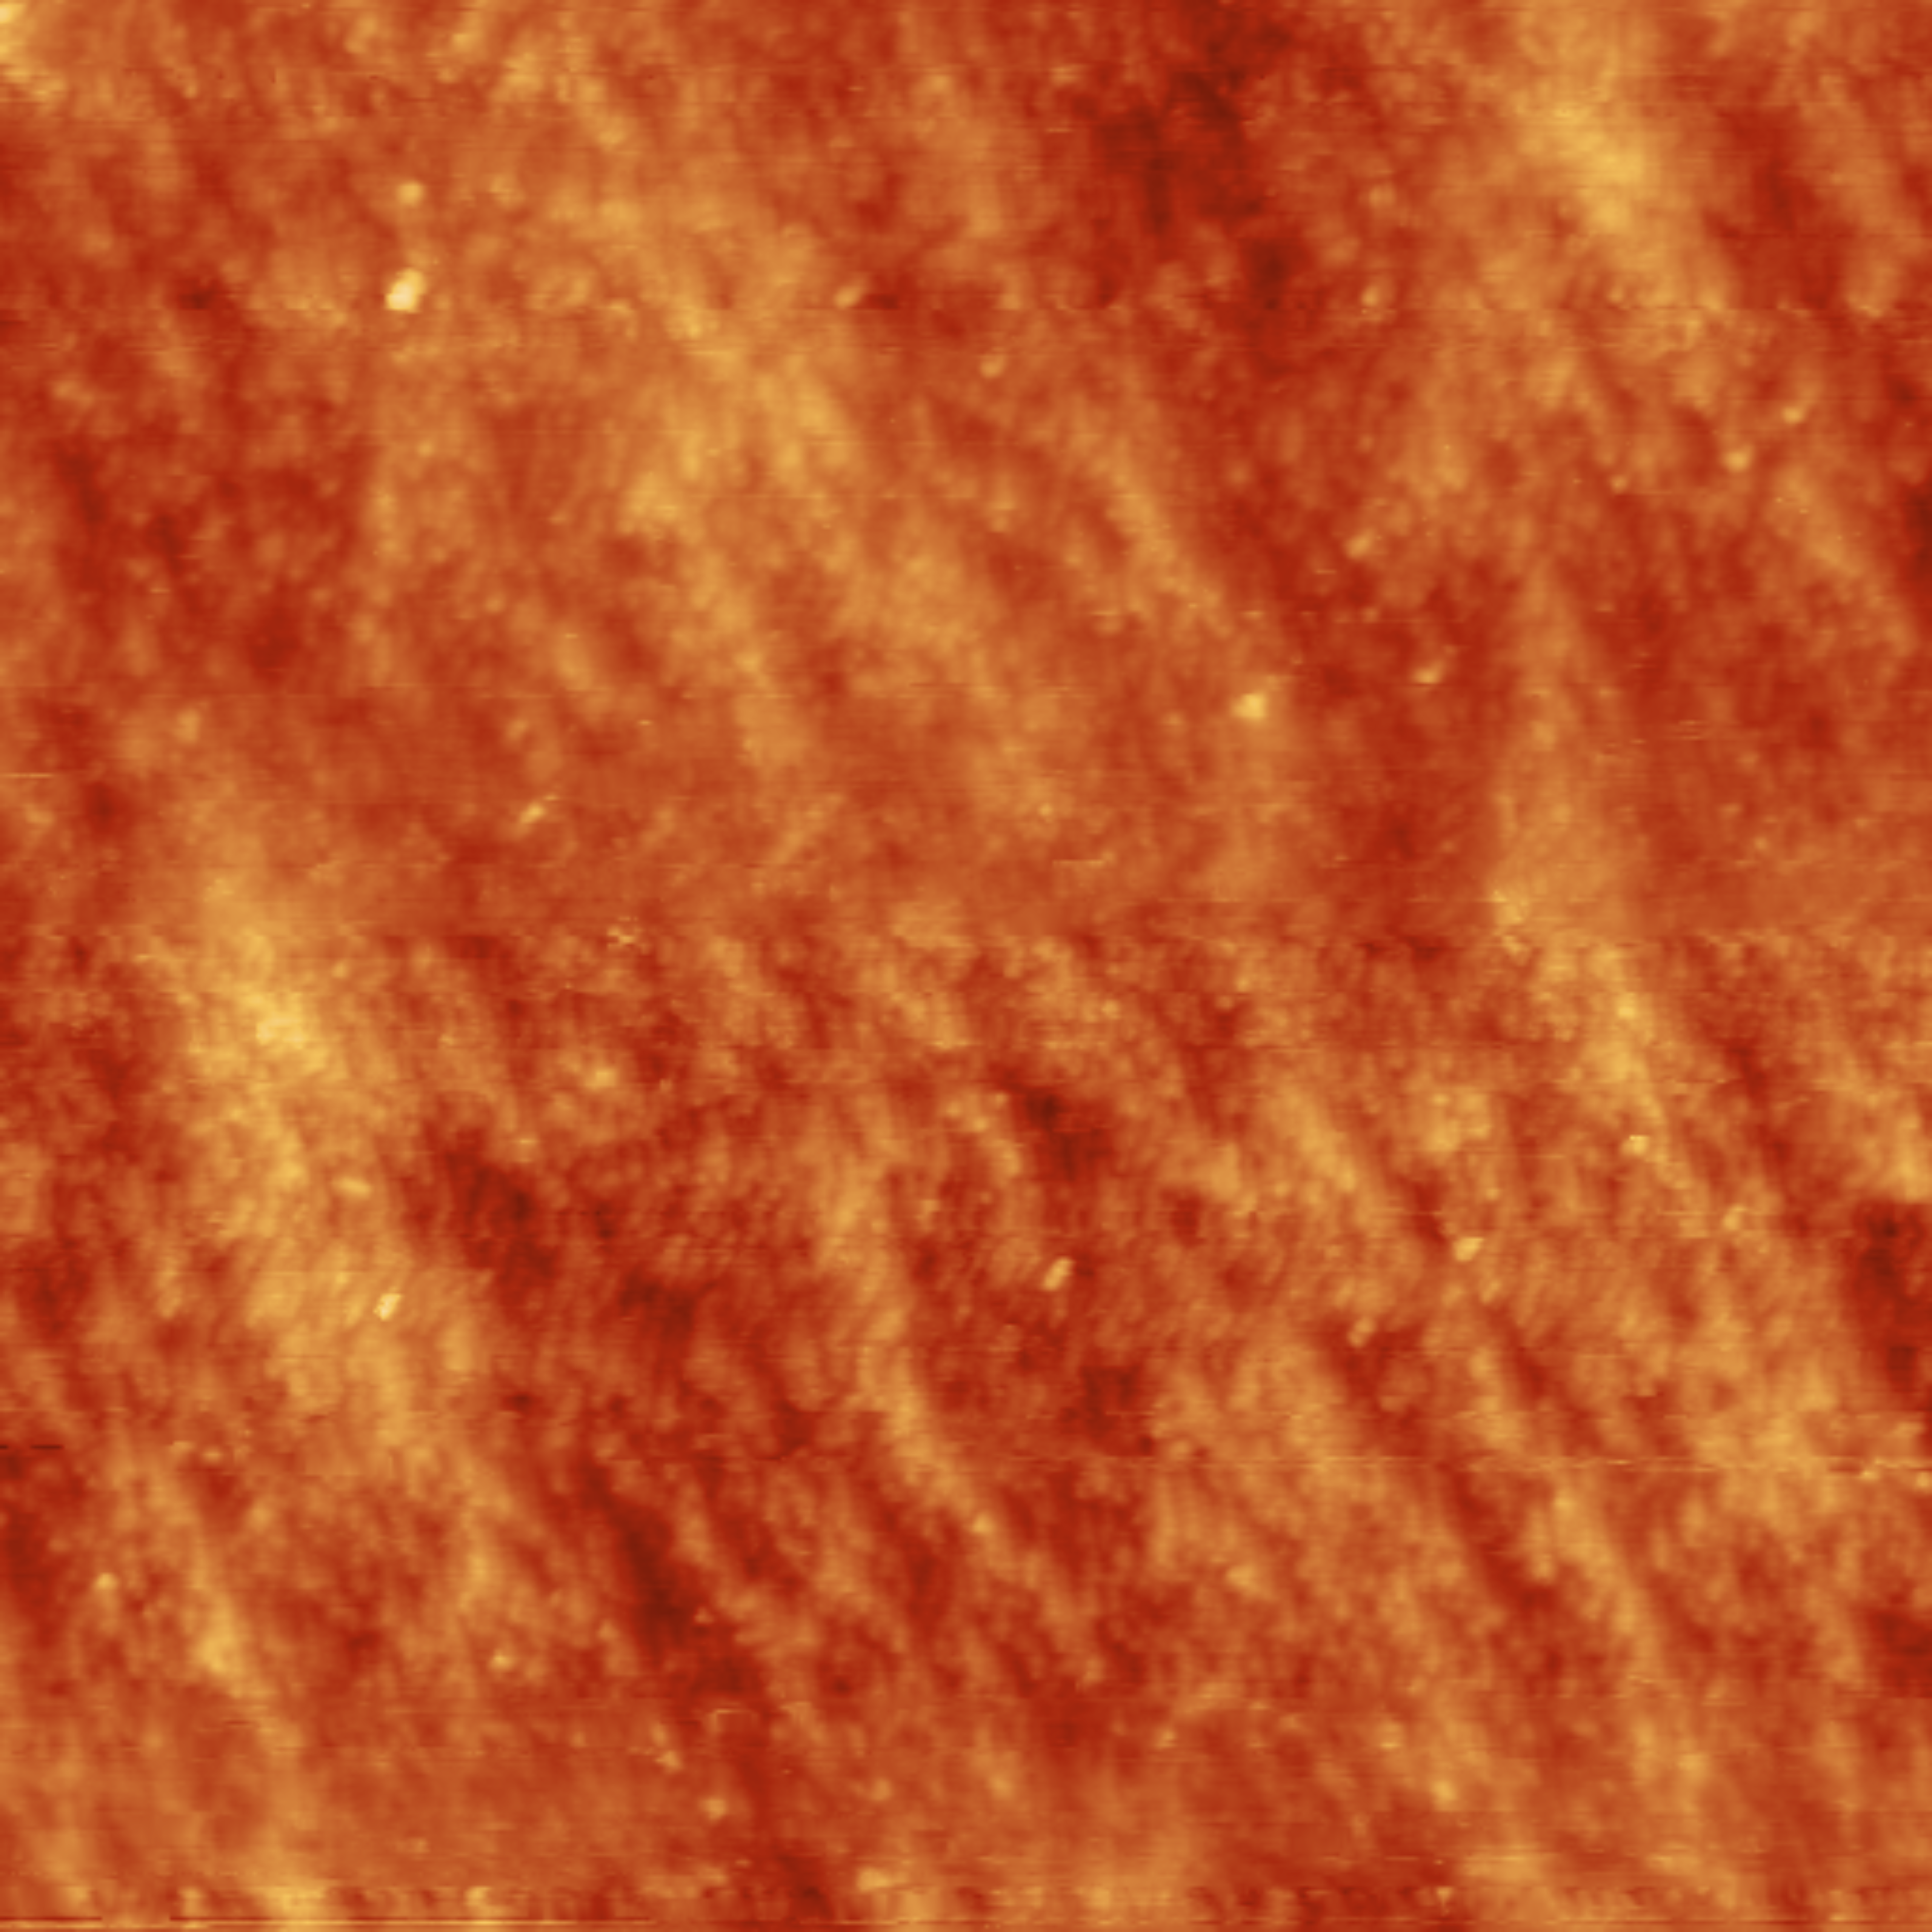
\includegraphics[width=0.45\textwidth]{./images/F150331-124839}
	%		\label{fig:30-31.03}
	%	}
	\subfigure[Cleaned copper foil before \textit{h}-BN growth. Surface shows many facets.
%	, the roughness is \SI{70}{\pico\meter}.
		]{%
		\includegraphics[width=0.5\textwidth]{./images/F150331-125720}
		\label{fig:cu-foil-clean-stm-1}
	} \quad
	%	\subfigure[STM image after \SI{4.5}{\langmuir} of borazine dosage on a \SI{750}{\celsius} hot copper foil surface. A small \textit{h}-BN island can be seen (lower right) on a largely uncovered copper foil background.]{%
	%		\includegraphics[width=0.45\textwidth]{./images/F150416-192611}
	%		\label{fig:F150416-192611}
	%	}
	%	\subfigure[STM image of \SI{22}{\langmuir} borazine dosed on a \SI{800}{\celsius} hot copper-foil surface. Several large islands can be seen that grow over Cu-foil step edges. Inset shows coverage with \textit{h}-BN ad layer in blue.]{
	%	\includegraphics[width=0.35\textwidth]{./images/F150423-102732-with-inset}
	%	\label{cu-foil-hBN-stm}
	%}
	\subfigure[Typical height profile. The roughness is \SI{70}{\pico\meter}.]{%
		\includegraphics[width=0.5\textwidth]{./images/F150331-125720-profile}
		\label{fig:cu-foil-clean-profile}
	}
	
	\caption{Cu-foil \subref{fig:cu-foil-clean-stm-1} after repeated sputtering and annealing cycles. \subref{fig:cu-foil-clean-profile} Height profile. Imaging parameters: \subref{fig:cu-foil-clean-stm-1} \SI{3.6}{\volt}, \SI{0.1}{\nano\ampere}, color scale \SIrange{0}{600}{\pico\meter}, Image width: \SI{88,6}{\nano \meter}, 
		%	\subref{fig:F150416-192611} \SI{1}{\volt}, \SI{0.37}{\nano\ampere}, color scale \SIrange{0}{900}{\pico\meter}, Image width: \SI{44,3}{\nano \meter}.
		%\subref{{cu-foil-hBN-stm}} \SI{4.7}{\volt}, \SI{0.2}{\nano\ampere}, color scale \SIrange{0}{7}{\nano\meter}, Image width: \SI{295}{\nano \meter}
	}
\label{fig:cu-foil-clean-stm}
\end{figure}
		
		
	\section{CVD-Growth of \textit{h}-BN with borazine}
	 \subsection{LT-STM characterization}
The foil was sputtered and annealed 4 times with temperatures of \SI{800}{\celsius}. Borazine was dosed at \SI{2e-7}{\milli \bar} for \SI{2.5}{\minute}. The sample was kept at \SI{750}{\celsius} for another 5 minutes after dosing. The sample was cooled down slowly. \autoref{fig:h-bn-overgrown-cu-1} shows some of the grown islands. The copper surface changes upon \textit{h}-BN growth and the terrace width increases below the \textit{h}-BN flakes. The typical faceting of the surface vanishes or can at least not be depicted because of the overgrowing \textit{h}-BN (\autoref{fig:h-bn-overgrown-cu-2}). 

	% -----------BILDER ---- DISKUSSION: 21.04
	%\begin{figure}
	% \centering
	% \includegraphics[width=0.7\textwidth]{./images/F150423-102732-with-inset}
	% \caption{}
	%\end{figure}
	%%%%%%%%%%%%%%%%%%%%%%%%%%%%%%%%%%%%%%%%%%%%%%%%%%%%%%%%%%%%%%%%%%%%%%%%%%%%%%%%%%%%%%%%%%
	%\begin{figure}
	% \centering
	%\subfigure[]{%
	%	\includegraphics[width=0.45\textwidth]{./images/F150416-192611-detail1.png}
	%	\label{fig:h-bn-overgrown-cu-1}
	%} \quad %
	%\subfigure[]{%
	%	\includegraphics[width=0.45\textwidth]{./images/F150423-114214.jpg} 
	% 	\label{fig:h-bn-overgrown-cu-2}
	%}%
	%\caption{STM topographies of \textit{h}-BN islands that overgrow Cu-foil facets. Imaging parameters: 		
	% 	\subref{fig:h-bn-overgrown-cu-1} 
	% 		\SI{1}{\volt}, \SI{0.37}{\nano\ampere}, 
	% 		color scale \SIrange{0}{1.5}{\nano \meter}, 
	% 		Image width: \SI{18}{\nano \meter}, 
	% 	\subref{fig:h-bn-overgrown-cu-2} 
	% 		\SI{3.5}{\volt}, \SI{0.5}{\nano\ampere}, 
	% 		color scale \SIrange{0}{4}{\nano \meter}, 
	% 		Image width: \SI{73,8}{\nano \meter}. 
	%}%
	%\label{fig:h-bn-overgrown-cu}
	%\end{figure}
	
The sample was sputtered and annealed several times to temperatures of \SI{800}{\celsius}. Before the dosage it was held 5 minutes at \SI{750}{\celsius}. Borazine was dosed with the same pressure as before (\SI{1e-7}{\milli \bar}) but for 1min and at a lower temperature of \SI{750}{\celsius}. After the preparation the sample was kept at \SI{750}{\celsius} for another 1 minute. It was cooled down slowly (shown in \autoref{fig:F150416-192611} and \autoref{fig:h-bn-overgrown-cu}).

	\begin{figure}[h!]
		\centering
		\subfigure[]{%
			\includegraphics[width=0.45\textwidth]{./images/F150423-102732}
			\label{fig:h-bn-22L}
		} \quad %
		\subfigure[]{%
			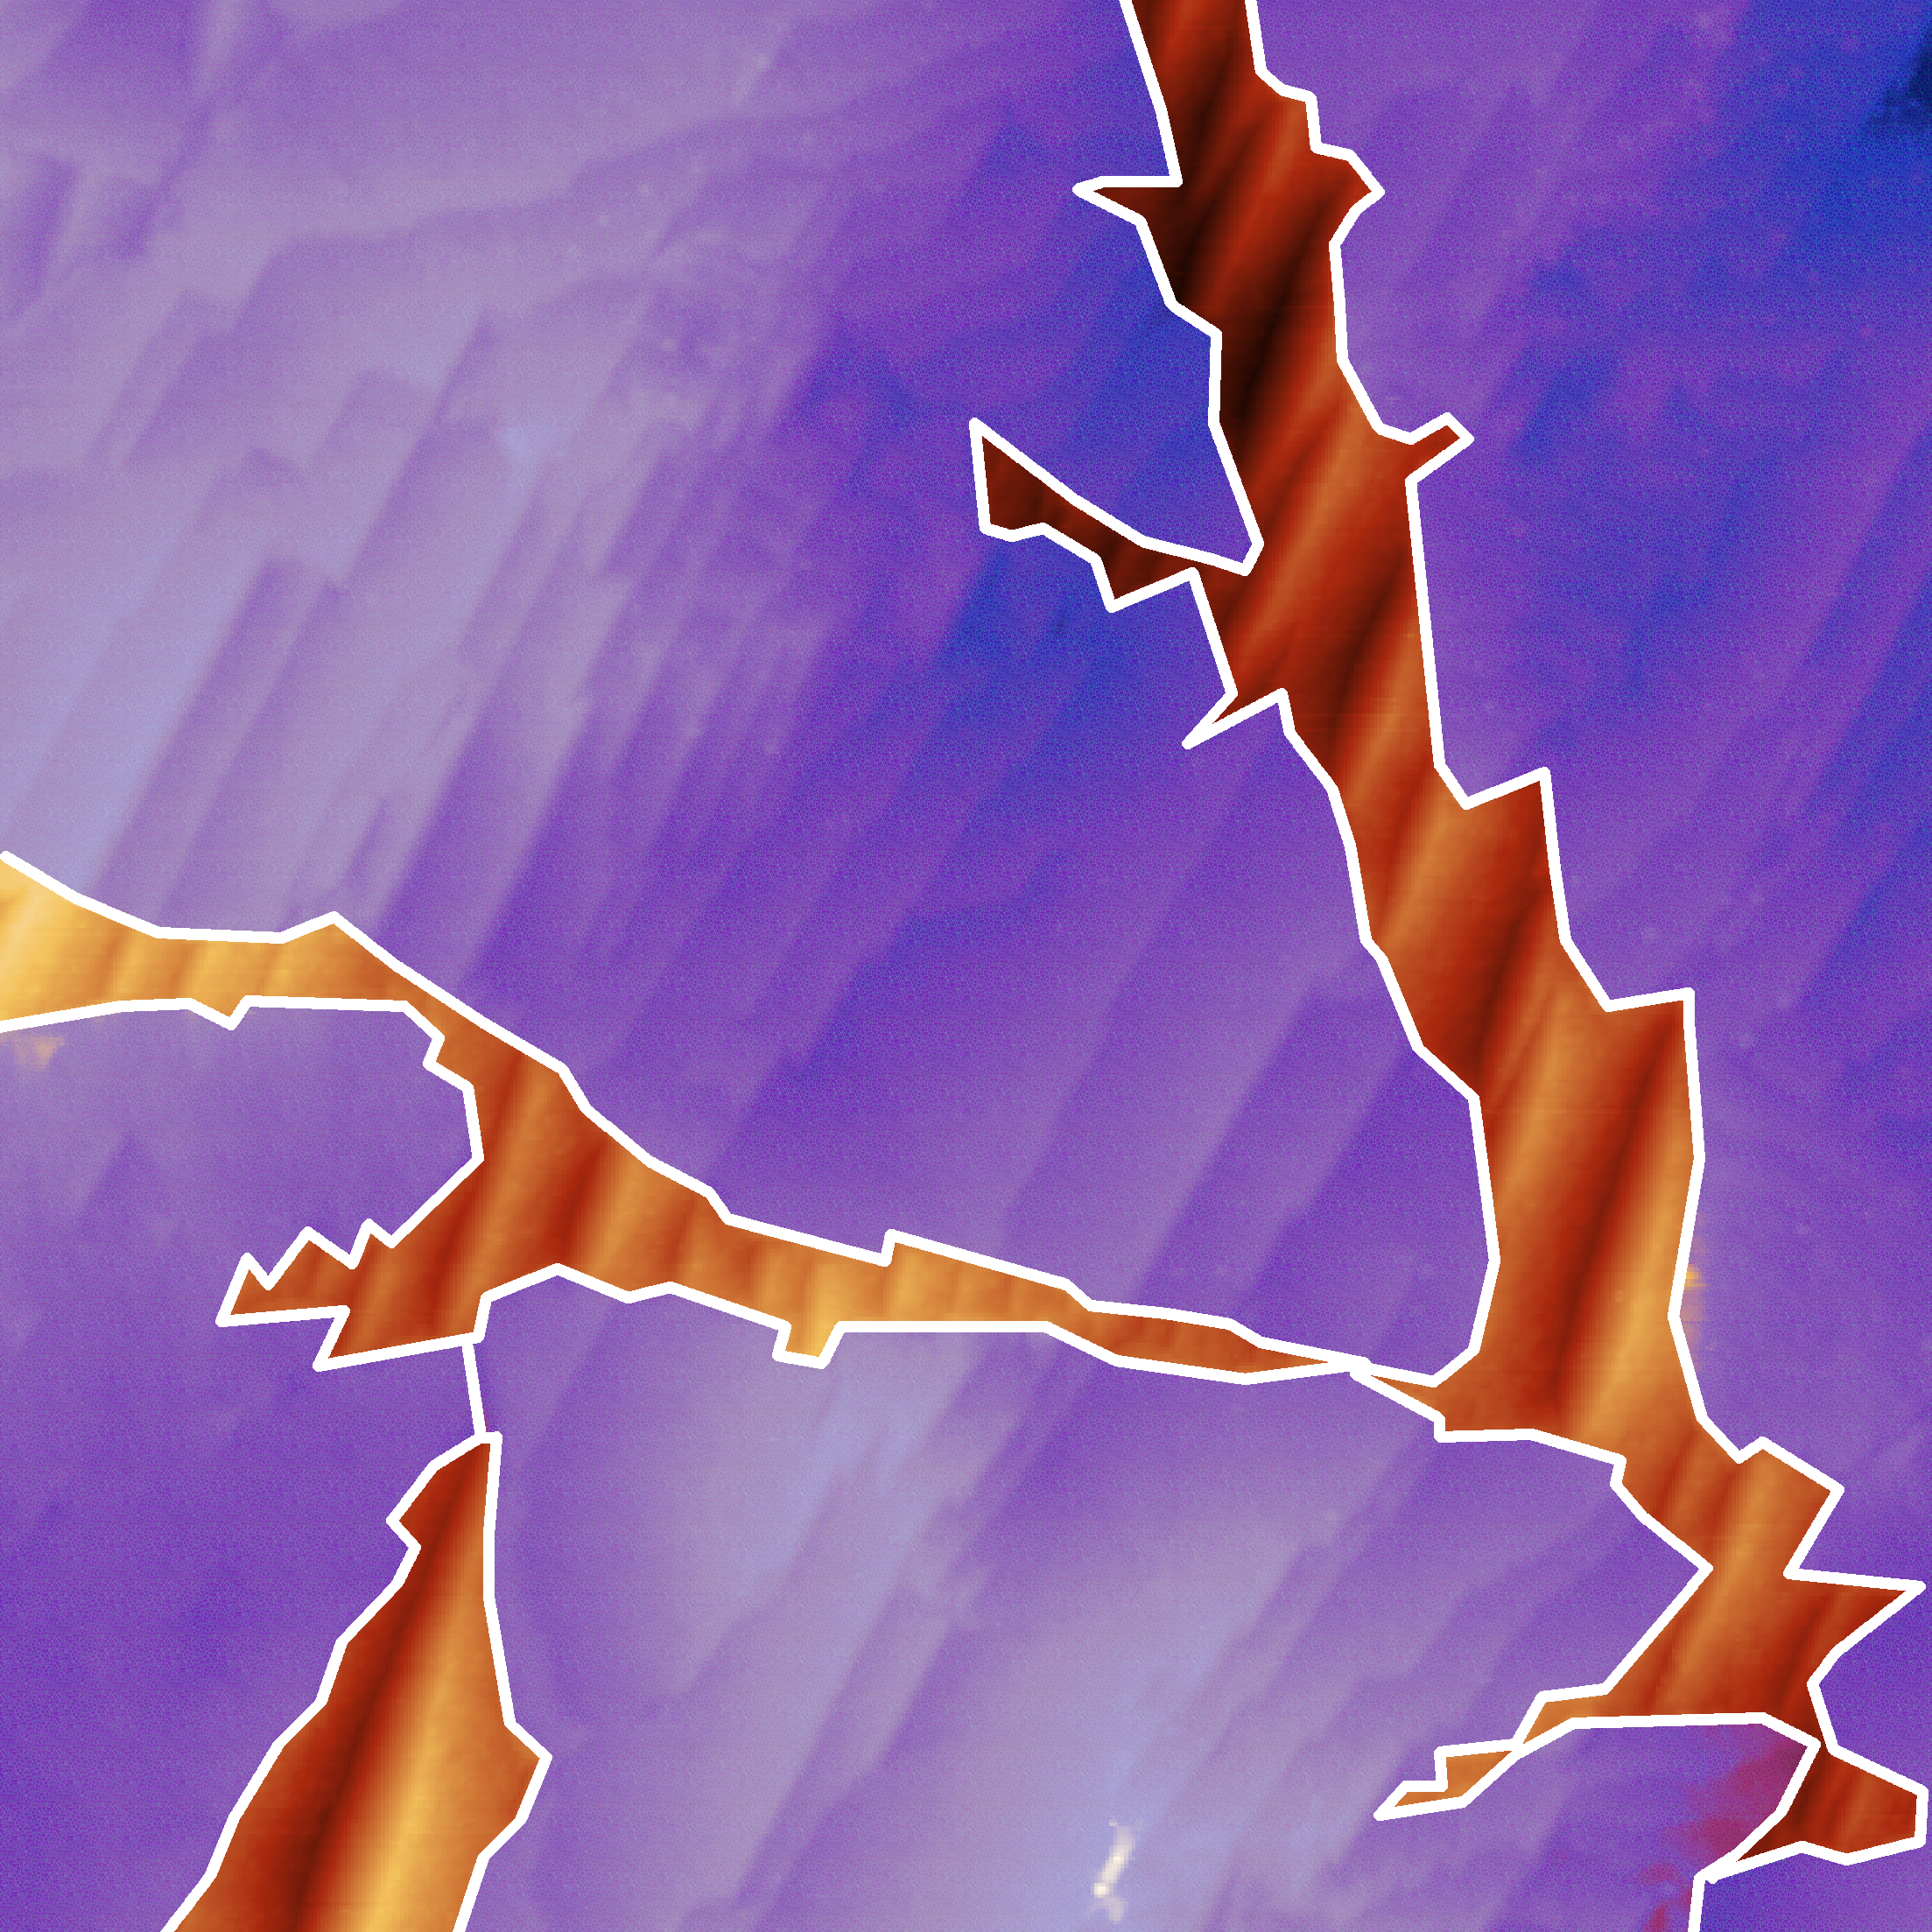
\includegraphics[width=0.45\textwidth]{./images/F150423-102732-overlayed.png} 
			\label{fig:h-bn-22L-2}
		}%
		\caption{STM topographies of \textit{h}-BN islands that overgrow Cu-foil facets. Imaging parameters: 		
			\SI{4.7}{\volt}, \SI{0.2}{\nano\ampere}, color scale \SIrange{0}{7}{\nano\meter}, Image width: \SI{295}{\nano \meter}
		}%
		\label{fig:h-bn-overgrown-cu}
	\end{figure}
	%%%%%%%%%%%%%%%%%%%%%%%%%%%%%%%%%%%%%%%%%%%%%%%%%%%%%%%%%%%%%%%%%%%%%%%%%%%%%%%%%%%%%%%%%%
%%%%%%%%%%%%%%%%%%%%%%%%%%%%%
\FloatBarrier
%%%%%%%%%%%%%%%%%%%%%%%%%%%%%

\subsection{XPS characterization}
%this file contains information on self-grown \textit{h}-BN on the comercially bought copper foils
Copper foils with \SI{0.25}{\mm} were bought and repeatedly sputtered/annealed. Several grow cycles of \textit{h}-BN via CVD of borazine were done.  The sample is transfered to the XPS-STM chamber and again sputtered/annealed several times to clean it properly.

The needed dosage of borazine to assemble a full mono layer of \textit{h}-BN is derived via a combined STM/XPS measurement. Several preparations were done to understand the growth behavior of \textit{h}-BN on the copper foil. Coverages are measured in STM while the chemical composition of the sample was assessed with XPS.
\begin{table}[h!]
	\centering
	\caption{Determination of the full mono layer borazine dosage. First a certainly saturated sample was prepared (I) and measured in XPS/STM. A sub-mono layer (II) was grown and compared to the monolayer STM and XPS results.}
	\begin{tabular}{cccccccc}
		& Prep. & Position    & Area [arb.u.] & FWHM  & Anode & Dosage  & Coverage\\ 
		&	  &	[eV]	& (XPS)		&[eV]	&Element&[L]	  & (STM) \\ \hline \hline
		\multirow{2}{*}{B1s} 	&I& 191.1 & 3776 & 1.35 & Mg & 4736 & \SI{100}{\percent}\\
		&II& 191.1 & 1994 & 1.35 & Mg & 789 &\SI{53}{\percent}\\ \hline
		\multirow{2}{*}{N1s} 	&I& 398.7 & 5875 & 1.45 & Al  & 4736 & \SI{100}{\percent}\\
		&II& 398.6 & 3183 & 1.43 & Al & 789 &\SI{54}{\percent}\\
	\end{tabular}
\end{table}

%\begin{figure}[ht]
%	\centering
%	\subfigure[N1s]{
%		\includegraphics[width=.45\textwidth]{./images/XPS-150314-N1s.jpg}
%	}
%	\subfigure[B1s]{
%		\includegraphics[width=.45\textwidth]{./images/XPS-150314-B1s.jpg}
%	}
%	\subfigure[C1s]{
%		\includegraphics[width=.45\textwidth]{./images/XPS-150314-C1s.jpg}
%	}
%	\subfigure[Cu3s]{
%		\includegraphics[width=.45\textwidth]{./images/XPS-150314-Cu3s.jpg}
%	}
%	\caption{\textbf{REDO! Axis too small!! Check layout with other XPS measurements!!} XPS spectra for ML \textit{h}-BN/Cu-foil. The peaks are at their expected positions\cite{kidambi_situ_2014} and show no additional features. No remnants of sulfur or remaining oxygen could be found.}
%	\label{fig:xps-self-grown}
%\end{figure}

\begin{figure}[ht]
	\centering
	\subfigure{
		\includegraphics[width=.45\textwidth]{./images/N1s-prepared}
	}
	\subfigure{
		\includegraphics[width=.45\textwidth]{./images/B1s-prepared}
	}
	\subfigure{
		\includegraphics[width=.45\textwidth]{./images/C1s-prepared}
	}
	\subfigure{
		\includegraphics[width=.45\textwidth]{./images/O1s-prepared}
	}
	\caption{XPS spectra for ML \textit{h}-BN/Cu-foil. The peaks are at their expected positions\cite{kidambi_situ_2014} and show no additional features. No remnants of sulfur or remaining oxygen could be found.}
	\label{fig:xps-self-grown}
\end{figure}

When comparing the resulting coverage (STM coverage/XPS signal) (II) to the (saturated) mono layer (I) one can derive the minimal amount of borazine needed to process a mono layer of \textit{h}-BN on the copper foil. Comparing the coverages of a sample grown with CVD, \SI{7E-6}{\milli \bar} for 15min (I) and one grown with CVD, \SI{3.5E-6}{\milli \bar} for 5min (II), shows that reducing the dosage by a factor of 6 does not reduce the coverage by a factor of 6, but just by a factor of 2. Therefore (I) features a full monolayer and (II) only half of it. It follows that a full monolayer may be achieved by dosing \SI{1500}{\langmuir} borazine on a \SI{800}{\degreeCelsius} hot copper foil surface. 
Because the growth rate may certainly not be linear (less and less free copper surface to decompose borazine into building fragments while the layer assembles) the given dosage is a minimum estimation to achieve the mono layer.

Even though a much larger amount for borazine (\SI{4736}{\langmuir}) than needed for a mono layer (\SI{1500}{\langmuir}) has been dosed, the maximum coverage did not exeed ne XPS signal of a mono layer. So the growth of \textit{h}-BN on copper foil is self-limited (as in the case of many \textit{h}-BN/metal systems) to a full mono layer. It is not possible to achieve layer growth with this type of preparation.

T and t dependence is not subject to investigation because the growth is supposed to follow the same mechanisms as on the single-crystal case. Quiet some investigation has been done, \cite{orlando_epitaxial_2012,preobrajenski_monolayer_2007-1} to understand this process.

\subsubsection{Commercial \textit{h}-BN sample}
The quality of the as-bought \textit{h}-BN on copper foils\cite{_graphene_2014} is examined in XPS. Results are shown in \autoref{fig:xps-bought}.
%%%%%%%%%%%%%%%%%%%%%%%%%%%% make it better looking? %%%%%%%%%%%%%%%%%%%%%%%%%%%%%%%%%%%%%
\begin{figure}[ht]
	\centering
	\subfigure{
		\includegraphics[width=.45\textwidth]{./images/N1s-bought}
	}
	\subfigure{
		\includegraphics[width=.45\textwidth]{./images/B1s-bought}
	}
	\subfigure{
		\includegraphics[width=.45\textwidth]{./images/C1s-bought}
	}
	\subfigure{
		\includegraphics[width=.45\textwidth]{./images/O1s-bought}
	}
	\caption{XPS spectra of as-bought \textit{h}-BN/Cu-foil sample\cite{_graphene_2014}. All spectra are taken at room temperature in as-bought state (black) and after annealing to \SI{630}{\K} (blue) and \SI{970}{\K} (red).}
	\label{fig:xps-bought}
\end{figure}

%
%\begin{landscape}
%	\begin{figure}
%		\includegraphics[angle=0,width=1.2\textwidth]{./images/XPS-spectra-as-bought.pdf}
%		\caption{}
%	\end{figure}
%\end{landscape}	

The XPS spectra shows contribution of different atomic species. There are peaks for the O-atoms (1s: \SIrange{529}{535}{\eV})), C-atoms (1s $\approx \SI{285}{\eV}$), N-atoms (1s $\approx \SI{398}{\eV}$), B-atoms (1s $\approx \SI{190}{\eV}$) and Cu-atoms ($3p_{1/2,3/2}$: \SIrange{70}{80}{\eV})). One would expect the shape of the 1s-peaks to be singlet-like (one peak, gauss shaped) and the 3p-peak to be a doublet (two close lying peaks with area-ratio 1/2:3/2=1:2).

There are different oxygen containing species expected to be present on the unprepared sample surface, including $CO$/$CO_2$, $CuO$/$Cu_2O$ and $H_2O$. They are possible surface contaminants due to sample storage under atmospheric conditions.
\paragraph{O1s}
Position varies with temperature. The signal at room temperature(black) stems from adsorbed water and CO. These desorb with increasing temperature(blue). When going to higher temperatures(red) this peak increases again and shifts to higher binding energies. Not present in self-grown \textit{h}-BN (\autoref{fig:xps-self-grown})

\paragraph{C1s}
The C1s Peak decreases with increasing temperature and retains its position. This has the same  reason as for the O1s peak (desorption of CO due to the heating). Some of the carbon remains on the surface - even at temperatures as high as \SI{970}{\K}.

\paragraph{N1s/B1s}
The nitrogen/boron peaks show some temperature related changes. There is little change upon annealing to \SI{630}{\K}, both peaks shrink, but stay almost constant in their position in binding energy (sightly shifted to lower binding energies by about \SI{0.2}{\eV}). Position is [N1s: \SI{398.1}{\eV} | B1s: \SI{190.2}{\eV}]. Further annealing leads to a intensity decrease.

\paragraph{Cu3p}
The copper peak exhibits an increase in area when increasing the temperature. This is because some of the water and CO adsorbate desorb and more and more copper is contributing to the signal. This peak is a doublet, so both signals come from the same chemical copper surrounding.


The $Cu(OH)_2$ O1s peak is expected to be at \SIrange{531.3}{531.7}{\eV}\cite{deroubaix_x-ray_1992} which may explain the shoulder of the O1s peak to higher binding energies (O\textit{1s} metal: \SI{531}{\eV}). Nitrates ($NO_3$) have binding energies in the range from \SIrange{532.5}{533.5}{\eV}\cite[45]{wanger_handbook_1979}. This would imply either an replacement of nitrogen with oxygen, or some kind of oxygen on top or below the the BN layer. As proven by Simonov et al. in \cite{simonov_controllable_2012} the atomic oxygen tends to replace the nitrogen in the \textit{h}-BN/Ir(111) system when it is annealed to \SI{600}{\degreeCelsius}. Thus it forms $B_{x}N_{y}O_{1-x-y}$ over-layers. The longer the oxidation time the higher the amount of replaced nitrogen. 

If this effect is responsible for the O\textit{1s} peak at high temperatures is questionable, since the oxygen has to be cracked somehow - where no process can be thought of (no catalytic cracking at metal surface possible - full ML, thermal energy to low to reach binding energies of $O_2$ (\textcolor{red}{\textbf{no citation here, nothing found - just a guess}})).

\textbf{An exchange of O with B or N would be easily visible in XPS (due to changed N/B surroundings. Not sure if the signal of oxygen is large enough for that. Check DATA - confirm maybe}

  \section{Application: Molecular functionalization with TPCN}
  %--------- This is TPCN on h-BN/Cu-foil !
  The Cu(111) support for the \textit{h}-BN growth is replaced by a polycrystalline copper foil. The goal is to achieve the same ordering of molecules on the \textit{h}-BN surface. The \textit{h}-BN layer has been prepared by a dose of \SI{5E-7}{\milli\bar} borazine for \SI{20}{\min} (\SI{4500}{\L}). During dosage the foil has been kept at \SI{820}{\celsius}.
  
  When a \textit{h}-BN spacer layer is introduced, the molecules decouple from the substrate, lowering their interaction with the afore-mentioned. This can be seen in a change of the molecules' footprint (rectangular $\rightarrow$ square).
  
  They do not form ordered networks (like chains or squares) and lie rather loosely on the \textit{h}-BN layer (\textcolor{red}{\textbf{compare 150807.142226.dat}}). They can easily be moved with the STM tip (\SI{1}{\volt}, \SI{10}{\nano \ampere}). In some areas, denser TPCN islands form. Here they lie right next to each other, slightly shifted to match the neighboring molecules and to achieve the dense packed regions. The same motif was already investigated in the same system \cite{urgel_controlling_2015}.
  
  During scanning (I=\SI{0.1}{\nA}, \SI{0.9}{\V} <U<\SI{1.3}{\V}) of a group of molecules, a single molecule could be pushed out of the group (compare figure \autoref{fig:TPCN-manipulation} in appendix). While the chain initially consisted of 3 molecules in a row, after scanning one of the molecular units moved to the left while the remaining two stay at their positions. A closer look to the moved molecule's geometry reveals deformation of the legs.\textcolor{red}{\textbf{More information or don't mention?}}
  
  It was shown that the imminic nitrogen species within a 2H-TPP molecule strongly interact a Cu(111) surface, thus orient along high symmetry directions.\cite{haq_clean_2011, buchner_diffusion_2011, gonzalez-moreno_following_2011, diller_self-metalation_2012, ditze_activation_2012,rojas_self-assembly_2010} 
  Rotation and diffusion are limited. \textcolor{red}{\textbf{What does this tell me?}}
 
 TPCN without added cobalt form similar pattern on the \textit{h}-BN/Cu-foil system (compare fig. 2b in \cite{urgel_controlling_2015}). Although the ordered areas were quiet rare, an arranged region has been found. Here the molecules are not strictly equidistant or -rotated which makes it difficult to give an accurate unit cell for this type of motif.
  %--------- Describe how the TPCN form that network on h-BN --------- 
  
  \paragraph{Adding Co}
  Introducing some cobalt (15min, $T_{sample}=\SI{90}{\celsius}$) in the system, this self-assembly changes as depicted in \autoref{fig:TPCN+Co-STM}. The molecules now form a regular 2D network. All molecules are rotated the same and point their CN functions towards each other. 
  
  \begin{figure}[!h]
  	\centering
%  	\subfigure[Zoomed view ($\SI{10}\times\SI{10}{\square\nm}$)]{
%  		\includegraphics[width=0.45\textwidth]{./images/F150814-090450_01}
%  	}
%  	\subfigure[($\SI{20}\times\SI{35}{\square\nm}$)]{
%  		\includegraphics[width=0.45\textwidth]{./images/F150814-090305-cut1}
%	  	\label{fig:TPCN+Co-STM-large}
%  	}

  	\subfigure[Image width: $\SI{22}\times\SI{17}{\square\nm}$]{
  		\includegraphics[angle=90,height=0.7\textwidth]{./images/F150814-090305-cut1}
	  	\label{fig:TPCN+Co-STM-large}
  	} 
  	\subfigure[Image width: \SI{10}{\nano \meter}]{
  		\includegraphics[angle=90,width=0.45\textwidth]{./images/F150814-090305-cut2-background}
  		\label{fig:TPCN+Co-STM-small}
  	} \quad
  	\subfigure[Model]{
  		\includegraphics[angle=90,width=0.45\textwidth]{./images/F150814-090305-cut2-2}
	  	\label{fig:TPCN+Co-STM-small-model}
  	}
  	\caption{Self-Assembled TPCN molecules after Co adsorption on \textit{h}-BN/Cu-foil. The two moir\'e hills are partially visible in \subref{fig:TPCN+Co-STM-large}, imaged at \SI{4.46}{\volt}, \SI{0.04}{\nano\ampere}. The cobalt atoms highlighted in \subref{fig:TPCN+Co-STM-small} sit right in between the TPCN molecules and facilitate a regular, ordered arrangement.}
  	\label{fig:TPCN+Co-STM}
  \end{figure}
  
Molecules arrange in a square unit cell with center-center distances of \SI{2.43 \pm 0.01}{\nano \meter}.
  
A Co atom connecting two neighboring molecules via their legs would result in a distance of \SI{2.81 \pm 0.01}{\angstrom} between the N terminated leg and the center of the cobalt atom. Typical binding distances for Co-NC are reported \cite{schlickum_metalorganic_2007, przychodzen_supramolecular_2006} and in good agreement.

Few signs for porphyrin metalization, neither many access cobalt ad atoms (additional bright spots in between the molecules) are observed. Similar binding mechanisms are derived for this system.\cite{urgel_controlling_2015}

%  \SI{2.3}{\nano \meter}. This leaves a little void space in between 4 TPCN molecule's legs, space where a Co atom may be located. This would result in a distance of \SI{1.5}{\angstrom} between the end of a TPCN leg (its N-center) and the center of the cobalt atom. Typical binding distances for Co-NC are reported \cite{schlickum_metalorganic_2007, przychodzen_supramolecular_2006} and in good agreement.
  
  %---------- Build models in blender for correct spacings etc. ---------
  
  
  \section{Summary \& Outlook}
  points to point out:
  \begin{itemize}
  	\item Look at Messzeit-April.ppt power point presentation
  	\item Stufenh\"ohe
  	\item Beschaffenheit der stufen/facetts $\rightarrow$ material transport mechanism/strength differs under the h-BN compared to the bare cu-foil surface.
  	\item Wechselwirkung BN-Wachstum und Facettenbildung
  	\item Warum sehe ich kein moir\'e?!? Spannungsabhängigkeit [4V/1V] siehe 121542
  \end{itemize}

  	\paragraph{not done yet - maybe future?}
  Some foil has been mechanically polished with 4k paper and several hours of Syton polishing. The roughness of these samples has been investigated also in AFM. These are comparable to the chemically polished ones, but are always slightly higher by $\approx 10\%$. Sometimes unwanted new scratches appear after mechanical polish.
  
  To further improve the quality of the foil, one can follow the documented recipe for annealing the foil in a $H_2$ atmosphere (\SI{10}{sscm}, \SI{1000}{\celsius}, 30min)\cite{kim_synthesis_2012} to increase the copper grain size and further smoothen the surface. We decided to further prepare the foils within the UHV chamber and skipped this step.